%% Preambel
\documentclass[conference,compsoc,final,a4paper,12pt]{IEEEtran}
\usepackage[utf8]{inputenx}

\newcommand{\autoren}[0]{Ahmed Salame, Ida Vanessa Gouleu Mokam}

\newcommand{\dokumententitel}[0]{Websockets mit Grails}

% Hie muss normalerweise nichts angepasst werden
\usepackage[pdftex]{graphicx}
\graphicspath{{img/}}
\DeclareGraphicsExtensions{.pdf,.jpeg,.png}
\usepackage[cmex10]{amsmath}
\usepackage{algorithmic}
\usepackage{array}
\usepackage{dblfloatfix}
\usepackage{url}
\usepackage[autostyle=true,german=quotes]{csquotes}
\usepackage[backend=biber]{biblatex}
\usepackage{booktabs}
\usepackage{xcolor}
\usepackage{listings}             % Source Code listings
\usepackage[printonlyused]{acronym}

% Farben definieren
\definecolor{linkblue}{RGB}{0, 0, 100}
\definecolor{linkblack}{RGB}{0, 0, 0}
\definecolor{darkgreen}{RGB}{14, 144, 102}
\definecolor{darkblue}{RGB}{0,0,168}
\definecolor{darkred}{RGB}{128,0,0}
\definecolor{comment}{RGB}{63, 127, 95}
\definecolor{javadoccomment}{RGB}{63, 95, 191}
\definecolor{keyword}{RGB}{108, 0, 67}
\definecolor{type}{RGB}{0, 0, 0}
\definecolor{method}{RGB}{0, 0, 0}
\definecolor{variable}{RGB}{0, 0, 0}
\definecolor{literal}{RGB}{31,0, 255}
\definecolor{operator}{RGB}{0, 0, 0}

\usepackage[ngerman]{betababel}
\usepackage[
	    unicode=true,
      hypertexnames=false,
      colorlinks=true,
      colorlinks=false,
      linkcolor=darkblue,
      citecolor=darkblue,
      urlcolor=darkblue,
      pdftex
   ]{hyperref}
%	 \PrerenderUnicode{ü}

% Einstellungen für Quelltexte
\lstset{
      xleftmargin=0.1cm,
      basicstyle=\scriptsize\ttfamily,
      keywordstyle=\color{keyword},
      identifierstyle=\color{variable},
      commentstyle=\color{comment},
      stringstyle=\color{literal},
      tabsize=2,
      lineskip={2pt},
      columns=flexible,
      inputencoding=utf8,
      captionpos=b,
      breakautoindent=true,
	  breakindent=2em,
	  breaklines=true,
	  prebreak=,
	  postbreak=,
      numbers=none,
      numberstyle=\tiny,
      showspaces=false,      % Keine Leerzeichensymbole
      showtabs=false,        % Keine Tabsymbole
      showstringspaces=false,% Leerzeichen in Strings
      morecomment=[s][\color{javadoccomment}]{/**}{*/},
      literate={Ö}{{\"O}}1 {Ä}{{\"A}}1 {Ü}{{\"U}}1 {ß}{{\ss}}2 {ü}{{\"u}}1 {ä}{{\"a}}1 {ö}{{\"o}}1
}

\hypersetup{
  pdftitle={\dokumententitel},
	pdfauthor={\autoren},
	pdfdisplaydoctitle=true
}

% Wo liegt Sourcecode?
\newcommand{\srcloc}{src/}

% Literatur einbinden
\addbibresource{literatur.bib}

\begin{document}

% Titel des Dokuments
\title{\dokumententitel}

% Namen der Autoren
\author{
  \IEEEauthorblockN{\autoren}
  \IEEEauthorblockA{
    Hochschule Mannheim\\
    Fakultät für Informatik\\
    Paul-Wittsack-Str. 10,
    68163 Mannheim
    }
}

% Titel erzeugen
\maketitle
\thispagestyle{plain}
\pagestyle{plain}
 % Weitere Einstellungen aus einer anderen Datei lesen

% Eigentliches Dokument beginnt hier
% ----------------------------------------------------------------------------------------------------------

% Kurze Zusammenfassung des Dokuments
\begin{abstract}
Dieses Paper soll aufzeigen, wie Websockets mit Grails realisiert werden kann. Zunächst wird auf einige Grundlagen näher eingegangen, um dem Leser ein Besseres Verständnis für das Thema zu vermitteln. 

--TODO--
\end{abstract}

\tableofcontents

\section{Einleitung}
 
\section{Forschungsmethode}

Beim Recherchieren wurde unter anderem Google Books \footnote{https://books.google.de/} verwendet, um passende Literatur zu finden. Des weiteren wurde die Homepage The Groovy Project herangezogen, um die Sprache Groovy näher zu beleuchten.
Zudem wurde nach passenden Quellen aus dem Internet gesucht, um bestimmte Themen näher zu erläutern. Zudem sind diese auch für jeden zugänglich. 

\section{State of the art}

Hier wird der Aktuelle Stand aufgezeigt


\section{Einleitung}

\section{Weiterer Titel}

\section{Fazit}
 
\begin{figure*}[h]
  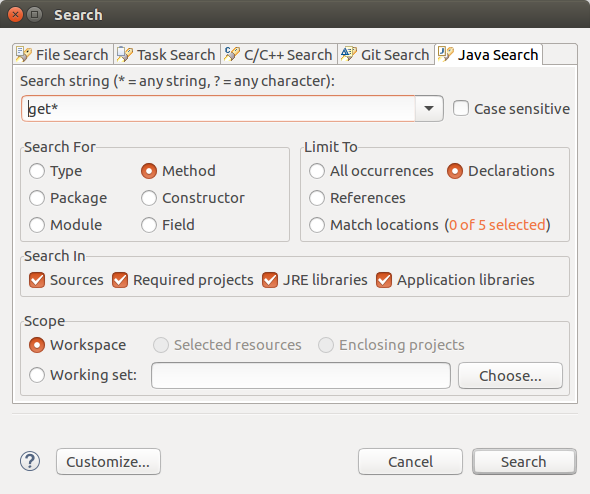
\includegraphics[width=\textwidth,height=7cm]{eclipse_suche.png}
  \caption{Beispiel einer Abbildung}
\end{figure*}

\begin{lstlisting}[language=Groovy,caption=Beispiel eines Listings]
class A{ 
	def a = 5
}
\end{lstlisting}

%--------------------------

\lstlistoflistings

\listoffigures

\section*{Abkürzungen}
\addcontentsline{toc}{section}{Abkürzungen}

\begin{acronym}
\acro{POJO}{Plain Old Java Object\emph{•}}
\acro{JTA}{Java Transaction API}
\acro{JSR}{Java Specification Request}
\end{acronym}

% Literaturverzeichnis
\addcontentsline{toc}{section}{Literatur}
\printbibliography

\end{document}